% ===========================================================================
\section{Experimental detail}
% ===========================================================================

\subsection{Cavity bodies and surface preparation}

Three copper bodies carry every measurement in this work: an eight-piece hexagonal prism, a two-piece hexagonal prism, and a cylinder of Braine's geometry~\cite{Braine:2024nzi} (Fig.~\ref{fig:threebodies}). All are oxygen-free high-conductivity (OFHC) copper.

\begin{figure}[htb]
    \centering
    \TODO{PHOTO: all three cavity bodies side by side at the same scale --- eight-piece hexagon disassembled, two-piece hexagon, and the cylinder. One orienting figure for the whole paper.}
    \caption{The three copper cavity bodies used in this work.}
    \label{fig:threebodies}
\end{figure}

The eight-piece hexagonal prototype was cut at the National High Magnetic Field Laboratory machine shop from annealed OFHC stock as six walls plus two endcaps. It stood \qty{75}{\milli\meter} tall with \qty{13}{\milli\meter} flat faces, and the wall thickness tapered from about \qty{2}{\milli\meter} at the face centre to below \qty{0.5}{\milli\meter} at the vertices. Twelve hand-tightened stainless 2-56 screws held it together, and two gold-plated SMA connectors on the top endcap provided antenna coupling.

Four two-piece hexagonal cavities were ordered from Xometry and machined from bulk OFHC 101 copper. Each is two hexagonal-prism halves, \qty{72}{\milli\meter} tall, with a \qty{12.25}{\milli\meter} face length and a minimum wall thickness of \qty{2}{\milli\meter}. Four hand-tightened stainless 4-40 screws and three alignment pegs close the assembly. Even with the pegs, a gap remained at the centre of the seam wide enough to admit a sheet of paper, which sets the scale of the residual RF leakage discussed below.

The cylindrical body is Braine's cavity used unmodified, so its geometry is that of Ref.~\cite{Braine:2024nzi}: \qty{11}{\giga\hertz} in TM$_{010}$ with an outer diameter under \qty{26}{\milli\meter}. \TODO{Take the remaining dimensions --- height, inner diameter, wall thickness, piece count, fasteners, antenna ports --- directly from Braine's thesis rather than restating them.} Only its surface preparation differs from the published work.

Surface preparation improved across the sequence, and it is the single variable that best tracks the measured copper $Q$:

\begin{enumerate}
    \item \textbf{Hand polish.} Progressive SiC paper (400--1200 grit), then diamond slurry (5--\qty{1}{\micro\meter}), then vibratory colloidal silica (\qty{0.05}{\micro\meter}) for the flat eight-piece pieces. For the two-piece hexagon the acute inner corners forced an adapted method: abrasive wrapped around an eraser, roughly one minute per face per grit, stopping at 1200 grit.
    \item \textbf{LLNL chemical etch.} The facility-standard stainless protocol, applied in sequence: soap, HCl, dichromate solution, and an antioxidant.
    \item \textbf{Low-temperature anneal.} \qty{250}{\degreeCelsius} for \qty{6}{\hour} in a positive-pressure argon tube furnace, evacuated to \qty{4e-5}{\torr} before argon backfill at \qty{0.2}{\liter\per\minute}, to raise the copper residual resistivity ratio.
    \item \textbf{Electropolish.} A 3:2 mixture of phosphoric acid and butanol at \qty{45}{\degreeCelsius}, held at the current plateau for \qty{10}--\qty{15}{\minute} with agitation at approximately \qty{500}{rpm}. Applied to the cylindrical cavity only, because the hexagon's acute inner corners do not present uniform current density to the bath. \TODO{Cathode material and geometry, plateau voltage and current density, electrolyte volume, and the resulting roughness with its measurement method.}
\end{enumerate}

\subsection{Coatings}

Two coating stacks were deposited, both on the same Ta/Nb foundation and both in the same Kurt J.\ Lesker UHV magnetron sputtering system used for coupon work~\cite{withanageRapidNbSn2021}.

\textbf{Ta/Nb only.} A \qty{500}{\nano\meter} Ta diffusion barrier and a \qty{750}{\nano\meter} Nb layer, both by DC magnetron sputtering onto a substrate at \qty{200}{\degreeCelsius}, terminating at Nb. Ta was deposited at \qty{60}{\watt} in \qty{10}{\milli\torr} Ar and Nb at \qty{250}{\watt} in \qty{8}{\milli\torr} Ar. \TODO{Substrate rotation, and whether the endcaps were masked.}

\textbf{Ta/Nb + Nb$_3$Sn (Nb-first Cu-Sn route).} The Ta/Nb stack above, followed by thermally evaporated Cu-33~at.\%~Sn deposited in steps with \qty{30}{\second} holds between increments, then a post-reaction at \qty{715}{\degreeCelsius} for \qty{3}{\hour} in the sputtering chamber, then removal of the residual Cu-Sn by ammonium persulfate (APS) etching. This is the recipe down-selected from coupon work for its lateral uniformity and its sharp Ta/Nb$_3$Sn interface, at the cost of a lower $T_c$ onset than the Cu-Sn-first routes \TODO{cite companion Cu-substrate paper}. The eight-piece wall used \qty{500}{\nano\meter} Ta, \qty{500}{\nano\meter} Nb, and \qty{5}{\micro\meter} Cu-Sn. The two-piece hexagon substituted a HiPIMS Ta barrier at \qty{800}{\volt} peak and a \qty{50}{\micro\second} duty cycle, giving about \qty{300}{\nano\meter} of Ta.

\textbf{Ta/Nb + Nb$_3$Sn (hot-bronze route).} \TODO{hot-bronze cavity recipe: Cu-Sn thickness and composition, substrate temperature during Nb sputtering, whether a post-reaction follows, whether an etch is needed}

Two limits of the deposition hardware shaped the outcome. The thermal evaporator has neither substrate rotation nor substrate heating, so Cu-Sn thickness on a concave hexagonal surface depends on the local angle to the source. The two-piece hexagon was also coated without a mask over the endcaps, because a mask adds height and risks contacting the heater during transfer. Both walls and endcaps therefore received Nb$_3$Sn.

\subsection{RF measurement}

A Keysight PNA vector network analyser measured all quality factors, with a range to \qty{20}{\giga\hertz}, \qty{10}{dBm} output, \qty{1}{\kilo\hertz} IF bandwidth, and 200 sweep points. Each sweep spanned three times the resonance full width at half maximum. Cavities were driven in weak transmission ($S_{21}$), with weak coupling verified by a reflection dip below \qty{1}{dB}. That condition keeps the loaded $Q_L$ within \qty{10}{\percent} of the unloaded $Q_0$. Values are reported as measured and labelled $Q_L$ or $Q_0$ throughout; where a $Q_0$ is inferred from a $Q_L$, the \qty{10}{\percent} coupling correction is stated explicitly.

Cavities mounted on the RF probe of Ref.~\cite{Braine:2024nzi} (Fig.~\ref{fig:ProbePPMSVNACavity}), built from non-magnetic G10, copper, brass, and beryllium-copper. A calibrated Cernox sensor on the top of the cavity confirmed thermal equilibrium between the top and bottom.

\begin{figure}[tb]
    \centering
    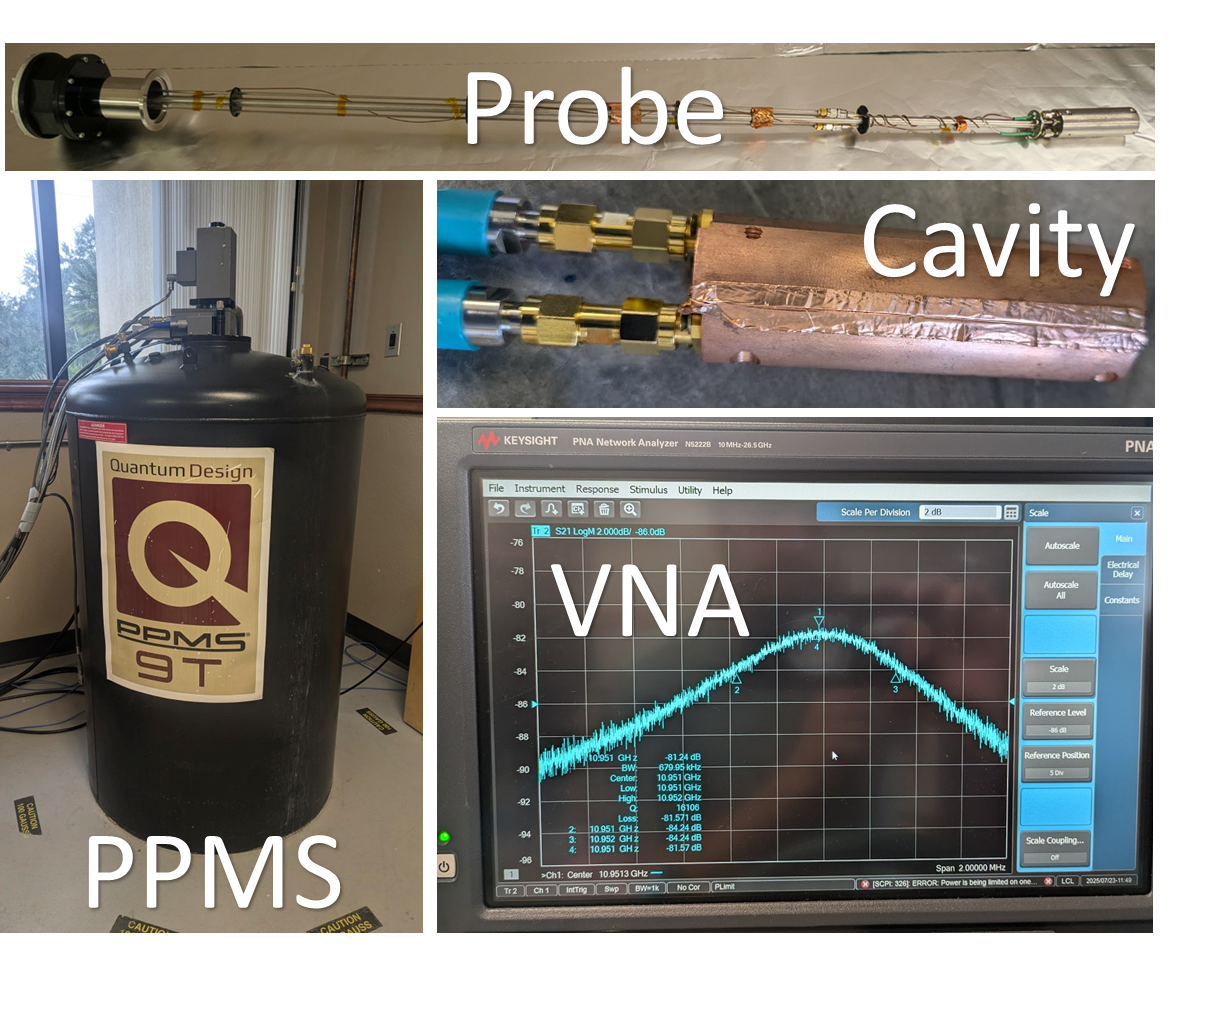
\includegraphics[width=0.9\linewidth]{images/AndreCavity/ProbePPMSVNACavity.png}
    \caption{Apparatus for $Q$ measurement: probe~\cite{Braine:2024nzi}, PPMS magnet, cavity, and VNA.}
    \label{fig:ProbePPMSVNACavity}
\end{figure}

Three measurement campaigns were run:

\textbf{$Q$ versus temperature (PPMS, \qty{2}{}--\qty{300}{\kelvin}).} The cavity cools to \qty{2}{\kelvin} in zero field, then $Q$ is recorded in \qty{0.5}--\qty{1}{\kelvin} steps through $T_c$, with one minute of equilibration after the PPMS stabilises. Below $T_c$ the residual resistance dominates. Above it, quasiparticles restore $R_\text{BCS}\propto \exp(-\Delta/k_BT)$ and $Q$ falls sharply, marking the film transition.

\textbf{$Q$ versus field (PPMS, \qty{0}--\qty{9}{\tesla} at \qty{2}{\kelvin}).} The field ramps in \qty{0.5}{\tesla} steps at the fastest available rate with a one-minute hold at each value, and the cavity axis stays parallel to the field. Below $H_{c1}$ the superconductor expels flux and $Q$ holds. Above it, vortices enter and oscillate under the RF drive, and the resulting Campbell resistance appears directly in $Q(B)$.

\textbf{$Q$ at millikelvin temperature (LLNL dilution refrigerator, \qty{50}--\qty{300}{\milli\kelvin}, zero field).} At these temperatures $R_\text{BCS}$ is exponentially suppressed, so what remains is the residual resistance from trapped flux, grain boundaries, surface oxides, and coating defects. The LLNL system follows the ASC protocol above. Field-dependent and millikelvin data were taken on separate systems because no available system delivers both, and the two are combined to estimate performance in haloscope conditions.
